\section{Verification Framework}
\label{sec:approach}

A verifier for these latent defects must (i) check the deployed
\textsc{Asl} artifact \emph{in place}, at build time, without a new
runtime; (ii) be \emph{sound where native}, when a property follows
from \textsc{Asl} alone, report only definite faults, so a CI gate can
block without triage; (iii) accept the omitted facts as \emph{semantic
premises} from sidecars, DSLs, or inference, grading severity by
provenance; and (iv) cover all six defect classes over \emph{one
representation} rather than as independent lints.
\tool{} separates the artifact being checked from the semantic facts available about it: a shared,
format-agnostic IR records the control flow and data movement that \asl{} exposes, and a layered
annotation slot records the contracts, business states, idempotency, persistence, and compensators
that \asl{} omits. Optional name/resource inference gives existing repositories a non-blocking
start, and severity tracks provenance (native and declared violations error, inferred facts warn).

\subsection{Architecture}
\label{sec:approach:arch}

\begin{figure}[t]
\centering
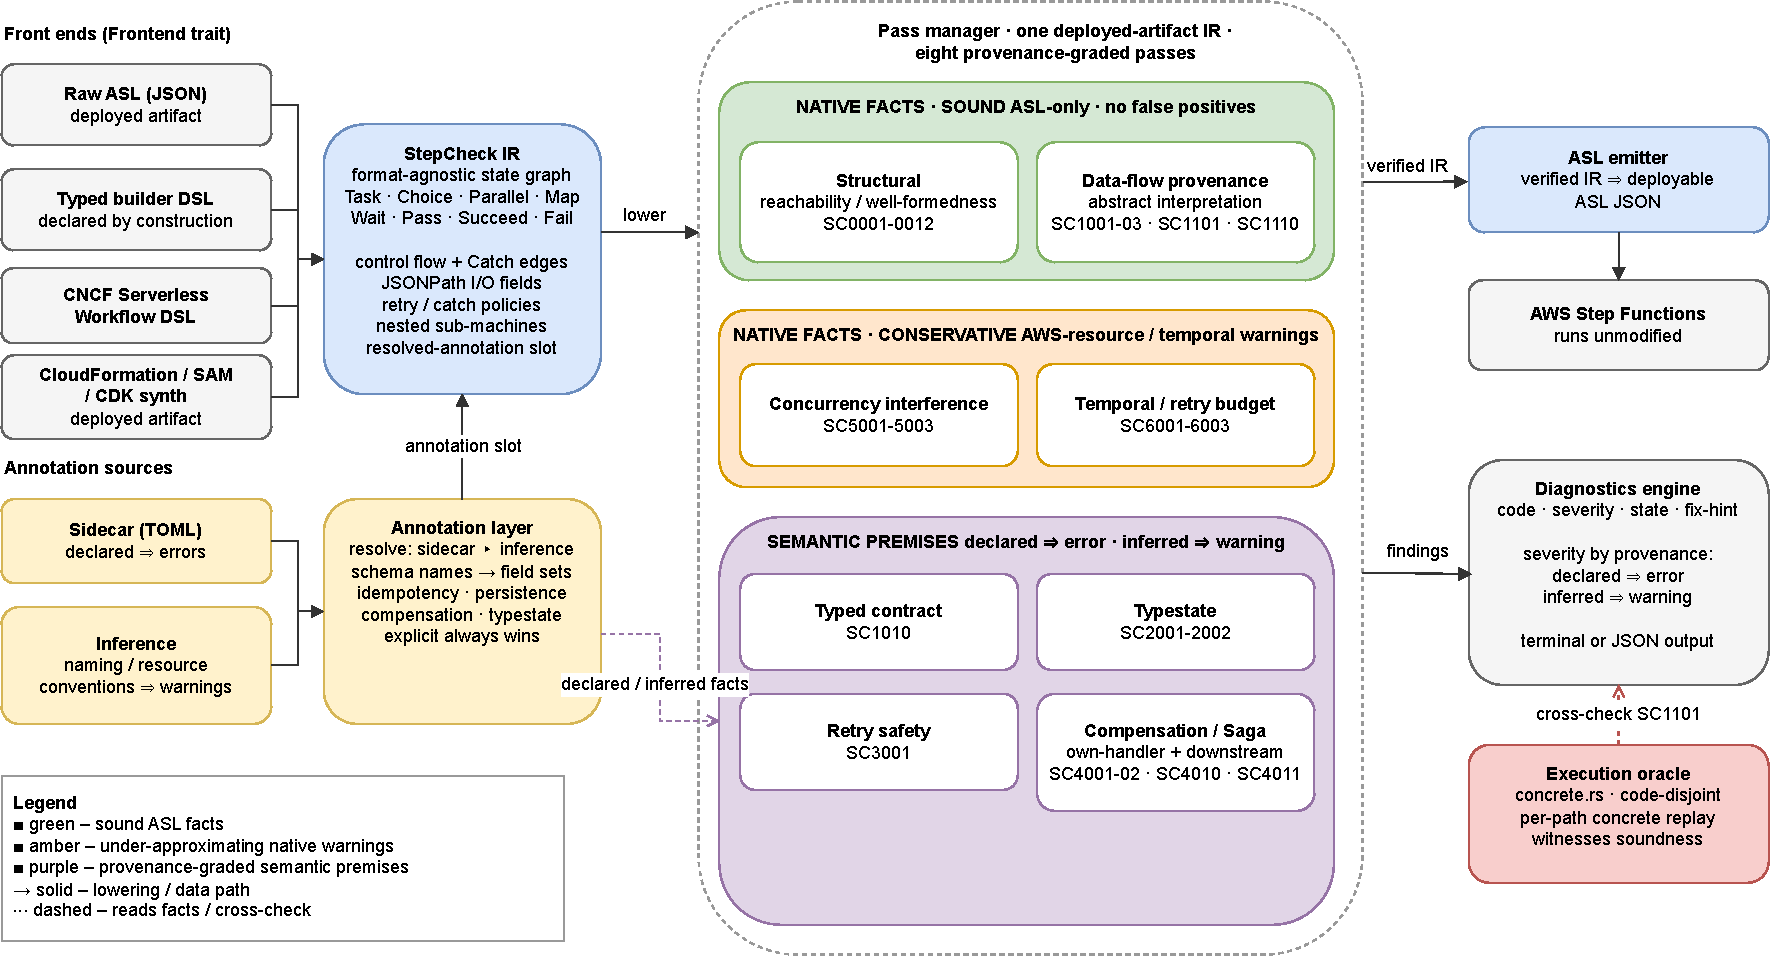
\includegraphics[width=\textwidth, height=6.5cm]{figures/figure3-architecture-detailed.pdf}
\caption{Verification pipeline: all front ends lower to one deployed-artifact IR shared by the
eight passes, rather than running independent lints.}
\label{fig:pipeline}
\end{figure}

Every front end lowers to the same workflow graph (Figure~\ref{fig:pipeline}); every analysis is
a pass over it; and the optional emitter lowers verified DSL-authored workflows back to deployable
\asl{}. Raw \asl{} is the primary input, parsed tolerantly through generic JSON, so intrinsics,
context references, SAM placeholders, dialect variants, and JSONata states never cause hard parse
failures. The typed DSL emits graph and annotations by construction, and the CNCF front end
exercises the same extension point.
The pass families are summarized in Table~\ref{tab:sccodes}. Native structural and data-flow checks
need only the \asl{} artifact. The \emph{conservative} concurrency and temporal checks report only provable conflicts
and may miss others---the opposite polarity to the over-approximating, sound data-flow analysis of
Section~\ref{sec:approach:dataflow}---and therefore warn, except the definite misconfiguration
\code{SC6003}. Semantic checks verify consistency with supplied premises; they do not prove those
premises true.

\emph{Structural and annotation hygiene} (\code{SC0001--0012}) is the base well-formedness layer:
it flags undefined targets, unreachable or dead-end states, non-exhaustive \texttt{Choice}, and
stale sidecar references. The remaining data-flow, concurrency, temporal, and declared-tier passes
are detailed in Sections~\ref{sec:approach:dataflow}--\ref{sec:approach:types}, and the technical
report~\cite{stepcheck-repo} tabulates the full pass-by-pass claim strengths. The IR itself is a recursive graph of named states with a designated start. Each state records its
\asl{} kind, normal successors, \texttt{Catch} edges, the five-stage I/O pipeline, retry and
timeout controls, JSONPath-vs-JSONata mode, nested \texttt{Map}/\texttt{Parallel} sub-machines, and
the annotation slot. This is enough for every pass; surface syntax stays in the front ends.

\begin{table}[tbp]
\centering\small
\setlength{\tabcolsep}{4pt}
\caption{Diagnostic codes by class, severity, and soundness tier: \emph{sound} (no false positives,
Thm.~\ref{thm:soundness}), \emph{conservative} (abstains rather than over-reports), \emph{declared}
(exact given annotations), \emph{advisory} (inferred, non-blocking).}
\label{tab:sccodes}
\resizebox{\textwidth}{!}{%
\begin{tabular}{@{}lllll@{}}
\toprule
Code(s) & Class & Severity & Tier & Required premise \\
\midrule
\code{SC0001}--\code{SC0010} & structural well-formedness & error/warn & sound & --- \\
\code{SC0011}/\code{SC0012} & sidecar consistency & error & declared & supplied sidecar \\
\code{SC1001}--\code{SC1003} & native data binding & error/warn & sound & valid ASL grammar \\
\code{SC1101} & data-flow field provenance & error/warn & sound & modeled fragment (else $\top$); \\
&&&&warn = inferred contract\\
\code{SC1110} & Choice-guard provenance & warning & conservative & modeled fragment (else $\top$) \\
\code{SC1010}/\code{SC2001}/\code{SC2002} & contracts / typestate & error & declared & declared schemas/protocol \\
\code{SC5001}--\code{SC5003} & concurrency interference & error/warn & conservative & static resource/child key \\
\code{SC6001}--\code{SC6003} & temporal bounds & error/warn & conservative & declared bounds \\
\code{SC4002}/\code{SC4011} & declared saga consistency & error & declared & declared compensator \\
\code{SC3001}/\code{SC4001}/\code{SC4010} & retry / compensation & error/warn & advisory/declared & inferred or declared effects \\
\bottomrule
\end{tabular}
}
\end{table}



\subsection{Native Data-Flow Verification}
\label{sec:approach:dataflow}

The native layer is a sound bug finder, not a complete verifier. If \tool{} reports \code{SC1101} as an error,
then under the modeled semantics of Theorem 1,
the referenced field is absent on every execution reaching that read. In inferred-contract mode, SC1101 downgrades to a warning meaning not guaranteed by the contract premise; the definite-absence reading and Theorem 1 apply to the native and declared closed-world tiers. 
If it is silent, the field may
still be absent for some inputs hidden behind $\top$. This is the right direction for a raw-artifact
checker facing arbitrary input and opaque task results.

The analysis tracks \emph{document and variable shapes}: either $\top$ (opaque: any field may be
present) or a finite record of fields that may occur. Joins union keys, with $\top$ absorbing; a
path is definitely absent when record descent reaches a missing key before $\top$. 
The transfer functions mirror the five-stage \textsc{Asl} I/O pipeline
and the \texttt{Assign}/\texttt{Catch} semantics: path stages re-root
the shape, constructors build closed records while checking
\texttt{.\$} reads, unknown task and sub-workflow results lift to $\top$
unless a declared output schema or a fixed AWS service envelope pins
their keys, and \texttt{ResultPath} merges results into the raw input
(full per-construct cases in~\cite{stepcheck-repo}).
For JSONata, \textsc{StepCheck} models direct \texttt{\$states.*} and
\texttt{\$var} references plus object-valued
\texttt{Output}/\texttt{Assign}/\texttt{Arguments} fragments;
unsupported expressions project to $\top$ and never produce
\texttt{SC1101}.
A forward iteration joins shapes along normal and \texttt{Catch} edges. Cycles can re-embed a
sub-document under a \texttt{ResultPath} and grow record depth without changing the key set, so
\tool{} applies depth-$k$ widening after every propagation step: any record nested deeper than $k$
(the implementation uses $k=12$) is replaced by $\top$. Widening is conservative---it can hide a
bug behind opacity, but it cannot manufacture a definite absence. 
With a finite key universe and bounded record depth, the lattice has
finite height, so the iteration terminates; a defensive round bound
lifts all entries to $\top$ rather than ever reporting from an
under-approximation (formula and telemetry in~\cite{stepcheck-repo}). In all experiments fixpoints converge
within 7 rounds.
The restock loop in Figure~\ref{fig:intro} illustrates why a fixpoint matters. \texttt{CheckStock}
has one incoming shape from \texttt{ReserveInventory} and one from the \texttt{WaitRestock}
back-edge; joining them keeps any loop-produced field alive, so \code{SC1101} fires on the
downstream \texttt{ChargeCard} read only because \emph{no} iteration produces \texttt{total}.

\begin{theorem}[Sound bug reports for missing-field references]\label{thm:soundness}
Under the modeled JSONPath/JSONata document-and-variable semantics, if \tool{} reports
\code{SC1101} as an error for a path $p$ at state $s$, then every concrete execution reaching $s$ lacks $p$ in
the document or variable selected by that read site, so the \asl{} runtime fails that reference. In
the native tier this holds for arbitrary execution input; in the typed tier it holds relative to the
closed-world reading of declared input schemas and, when result-shape modeling is enabled, declared
task-output schemas and fixed AWS service-result envelopes. Expressions outside the modeled fragment
lift to $\top$ and are therefore silent.
\end{theorem}

\begin{proof}[Proof sketch]
Let $\gamma$ map each abstract shape to the concrete JSON values it may
denote, with $\top$ denoting all values and records exactly their listed
keys. Every transfer function over-approximates the corresponding
\textsc{Asl} operation under $\gamma$; joins are least upper bounds and
depth-$k$ widening only replaces sub-records by $\top$, hence is
extensive, so the forward iteration computes a post-fixpoint
over-approximating every concrete environment reaching each state,
including all loop iterations. If lookup of $p$ at the read site reaches
a missing key before $\top$, no value in the concretization contains
$p$, so the modeled \textsc{Asl} read fails on every execution reaching
$s$; expressions outside the modeled fragment reach $\top$ and cannot
trigger the premise. The full proof, with per-construct
transfer-function cases, is in~\cite{stepcheck-repo}.
\end{proof}
The guarantee is relative to the modeled fragment, not verified against
AWS's implementation; unmodeled expressions lift to $\top$ and stay silent
by construction, the execution oracle finds zero counterexamples across
all reports, and differential validation of the model is future work.
\code{SC1110} applies the same definite-absence judgment
to \texttt{Choice} guards but stays a warning outside Theorem~\ref{thm:soundness}: rule
reachability depends on earlier guards such as \texttt{IsPresent}, so it marks a provably dead or
risky branch rather than an unconditional runtime fault.

\vspace{-0.25cm}
\subsection{Concurrency and Temporal Analyses}
\label{sec:approach:conservative}

The concurrency and temporal passes are conservative engineering checks. \texttt{Parallel} branches
and concurrent \texttt{Map} iterations receive document copies, so only external resources can
race. \tool{} records statically known resource keys (\texttt{TableName}, \texttt{QueueUrl},
\texttt{Bucket}, and other named targets; full list in~\cite{stepcheck-repo}). It emits \code{SC5001}
only for provably overwriting operations---\texttt{PutItem}/\texttt{PutObject} and statically named
\texttt{states:startExecution} collisions---leaving keyed, append-only, and compute-only operations
silent.
The temporal pass checks resilience knobs the platform does not cross-check. \code{SC6001} warns
when a callback or Activity task lacks a timeout or heartbeat and can wait to the platform maximum.
\code{SC6002} warns when a retry budget can exceed the machine timeout. \code{SC6003} errors on the
definite misconfiguration \texttt{HeartbeatSeconds}\,$\geq$\,\texttt{TimeoutSeconds}.

\vspace{-0.25cm}
\subsection{Semantic Verification}
\label{sec:approach:types}

The semantic layer consumes task facts \asl{} does not contain: a contract $T:A\rightarrow B$
(fields consumed and produced), a typestate transition
$s_{\mathrm{in}}^T\rightarrow s_{\mathrm{out}}^T$ in protocol $\delta$, idempotency (whether a retry
repeats an external effect), and persistence with an optional compensator. These are premises
(Section~\ref{sec:approach:annot}); \tool{} checks the workflow relative to them.

\vspace{-0.25cm}
\begin{proposition}[Declared-tier consistency]\label{prop:typecheck}
For a fully declared workflow $W$, \code{SC1010}/\code{SC2001}/\code{SC2002} emit no finding iff
every normal-flow task adjacency $T_1\to T_2$ satisfies
$\mathit{in}(T_2)\subseteq\mathit{out}(T_1)$ and
$s_{\mathrm{out}}^{T_1}=s_{\mathrm{in}}^{T_2}$, and every task transition belongs to the declared
protocol $\delta$. On the series-parallel fragment, this edge condition is equivalent to a standard
field/typestate typing judgment. Completeness is relative to the supplied annotations.
\end{proposition}

Here $\mathit{out}(T_1)$ is $T_1$'s declared output set---including fields it forwards, not only
those it computes---and $\mathit{in}(T_2)$ is $T_2$'s declared input set; under this closed-world
convention the edge-local check does not false-positive on a field merged upstream and passed
through. The checks are edge-local: a ship-before-pay reordering in the order workflow yields
typestate mismatches plus field-contract misses. Retry-safety is likewise premise-relative: a broad
\texttt{States.ALL}/\texttt{States.TaskFailed} retry of a task declared non-idempotent is
\code{SC3001}, while retries narrowed to specific transient classes are left alone.
Per-task checks (\code{SC4001}/\code{SC4010}) can see
that a persistent task has no compensating path, but they miss a later state failing after the
effect has committed. For a declared persistent task $P$ with compensator $C$, \code{SC4011} scans
the post-commit region reachable from $P$ before $C$ and asks whether every fallible state's generic
failure routes through a broad \texttt{Catch} to $C$, and whether no normal path reaches
\texttt{Fail} while bypassing $C$.
The declared Saga model assumes a single post-commit fault, feasible
normal paths, a unique generic catcher for \texttt{States.TaskFailed},
and linear handlers whose reachability to $C$ means execution of $C$.
\begin{theorem}[Relative soundness and completeness of the compensation check]\label{thm:saga}
For a workflow with declared persistence and compensators, under the declared Saga model,
\code{SC4011} emits no finding for persistent task $P$ with compensator $C$ iff every modeled
post-commit failure after $P$ executes $C$. Thus \code{SC4011} is sound and complete relative to
the declared model.
\end{theorem}
Outside these assumptions, \code{SC4011} remains a reachability check but is no longer sound or
complete. The model-independent \code{SC4001}/\code{SC4010} checks still flag any persistent effect
with no compensating path. Coverage therefore degrades to the per-task tier rather than going
silent; the built-in and corpus sagas satisfy the assumptions.

\vspace{-0.25cm}
\subsection{Recovering Workflow Semantics}
\label{sec:approach:annot}
\label{sec:approach:infer}

Declared facts enter through a sidecar for existing \asl{} or the typed DSL for greenfield workflows;
once declared they support error-level findings, and where absent the declared-tier checks are
silent.
Concrete sidecar syntax is deferred to the technical report~\cite{stepcheck-repo}; the analyses
use only the declared idempotency, persistence, compensation, and typestate facts.
The order saga's complete sidecar is 68 lines of TOML---about eight per-task lines over four tasks,
plus shared schema and protocol blocks---and the typed DSL emits the same facts by construction.
Optional inference gives existing repositories a zero-effort warning mode: read-like names imply
idempotent, write-like non-idempotent, resource-acquiring persistent, and notifications
non-idempotent but not persistent; with no signal it abstains, and explicit annotations override it.
Stale sidecar and schema references are caught syntactically (\code{SC0011}/\code{SC0012}). The
residual risk, semantic drift between a declared premise and the deployed Lambda, is outside
\tool{}'s scope; generating the sidecar from code or IaC keeps declared facts in sync.
